\documentclass[a4paper, 10pt, fleqn]{article}

\usepackage[utf8]{inputenc}
\usepackage[T1]{fontenc}
\usepackage{textcomp}
\usepackage{lmodern}
\usepackage[ngerman]{babel}
\usepackage{enumerate}
%\usepackage[landscape]{geometry} %for horizontal aligned documents

\usepackage{amsmath}
\usepackage{graphicx}

\usepackage{hyperref}
\usepackage{color}
%for displaying source code
\usepackage{listings}
\lstset{
                basicstyle=\footnotesize,
                keywordstyle=\color{blue},
                stringstyle=\color{red},
                commentstyle=\color{green},
}

\usepackage{float}

%macro definitions
\definecolor{shadecolor}{RGB}{200,200,200}
%command \cbox to define colored bg
\newcommand{\cbox}[1]{\par\noindent\colorbox{shadecolor}
{\parbox{\dimexpr\textwidth-2\fboxsep\relax}{#1}}}

%set document specific content
\title{Titel}
\author{Daniel Foehn}
\date{\today} %Es kann ein bestimmtes Datum eingetragen werden
\begin{document}
	\maketitle
	\tableofcontents
	\listoffigures
	\listoftables
	
	\section{Einleitung}
		\subsection{Andwendungszweck des Dokumentes}
		
		\subsection{Zielpublikum}
		
		\subsection{Versionierung}
		
		\subsection{Glossar}
	
	\clearpage
	\section{Übersicht}
	    \subsection{Systemkontext}
		%Width context diagram
		
		\subsection{Ausgangslage}
		
	\clearpage
	\section{Anforderungen}
		Es gilt ein Netzwerkfähiges Computerspiel mit dem Namen Dots\&Boxes zu entwickeln.
		\subsection{funktionelle Anforderungen}
			\begin{itemize}
				\item Gegen Computer spielbar
				\item Spielstand kann abgespeichert werden
				\item Spielstand kann vom Speicherstand geladen werden
				\item Es kann online nach einem NON-AI Gegenspieler gesucht werden
				\item Es werden die Regeln von Dots\&Boxes angewandt
			\end{itemize}
		\subsection{nicht-funktionelle Anforderungen}
			\begin{itemize}
				\item Es soll keine Angabe der IP Adresse nötig sein.
				\item Der Code soll gut und brauchbar dokumentiert sein
				\item Das GUI besteht aus
				\begin{itemize}
					\item Spielfeld
					\item Ersichtlich wer am Zug ist
					\item Linien können Spieler zugewiesen werden
					\item Das Spielfeld kann in Länge und Höhe variieren
				\end{itemize}
			\end{itemize}
	
	\clearpage
	\section{Zeitplanung}
		Abgabe ist in der letzten Semesterwoche (\textbf{18. Dez 2015})
	
	\clearpage
	\section{Testplanung}
		\subsection{Testumgebung}
		
		\subsection{Testfälle}
			 \subsubsection{Unit Tests}
			 
			  \subsubsection{Blackbox Tests}
			  
	\clearpage
	\section{Grobdesign}
		\subsection{Design of Punkt XY}
		%Lisitng of design aspects, not going far into detail
		%exp. GUI layout, Function Videocamera
		
	\clearpage
	\section{Detaildesgin}
		\subsection{Umsetzung von Punkt XY}
		%lisitng of implementation details
		%incl. class and sequence diagram
		\subsection{Zustandsdiagramm}
		
		\subsection{Sequenzdiagramm}	
		
		\subsection{Klassendiagramm}
			\begin{figure}[H]
				\centering
				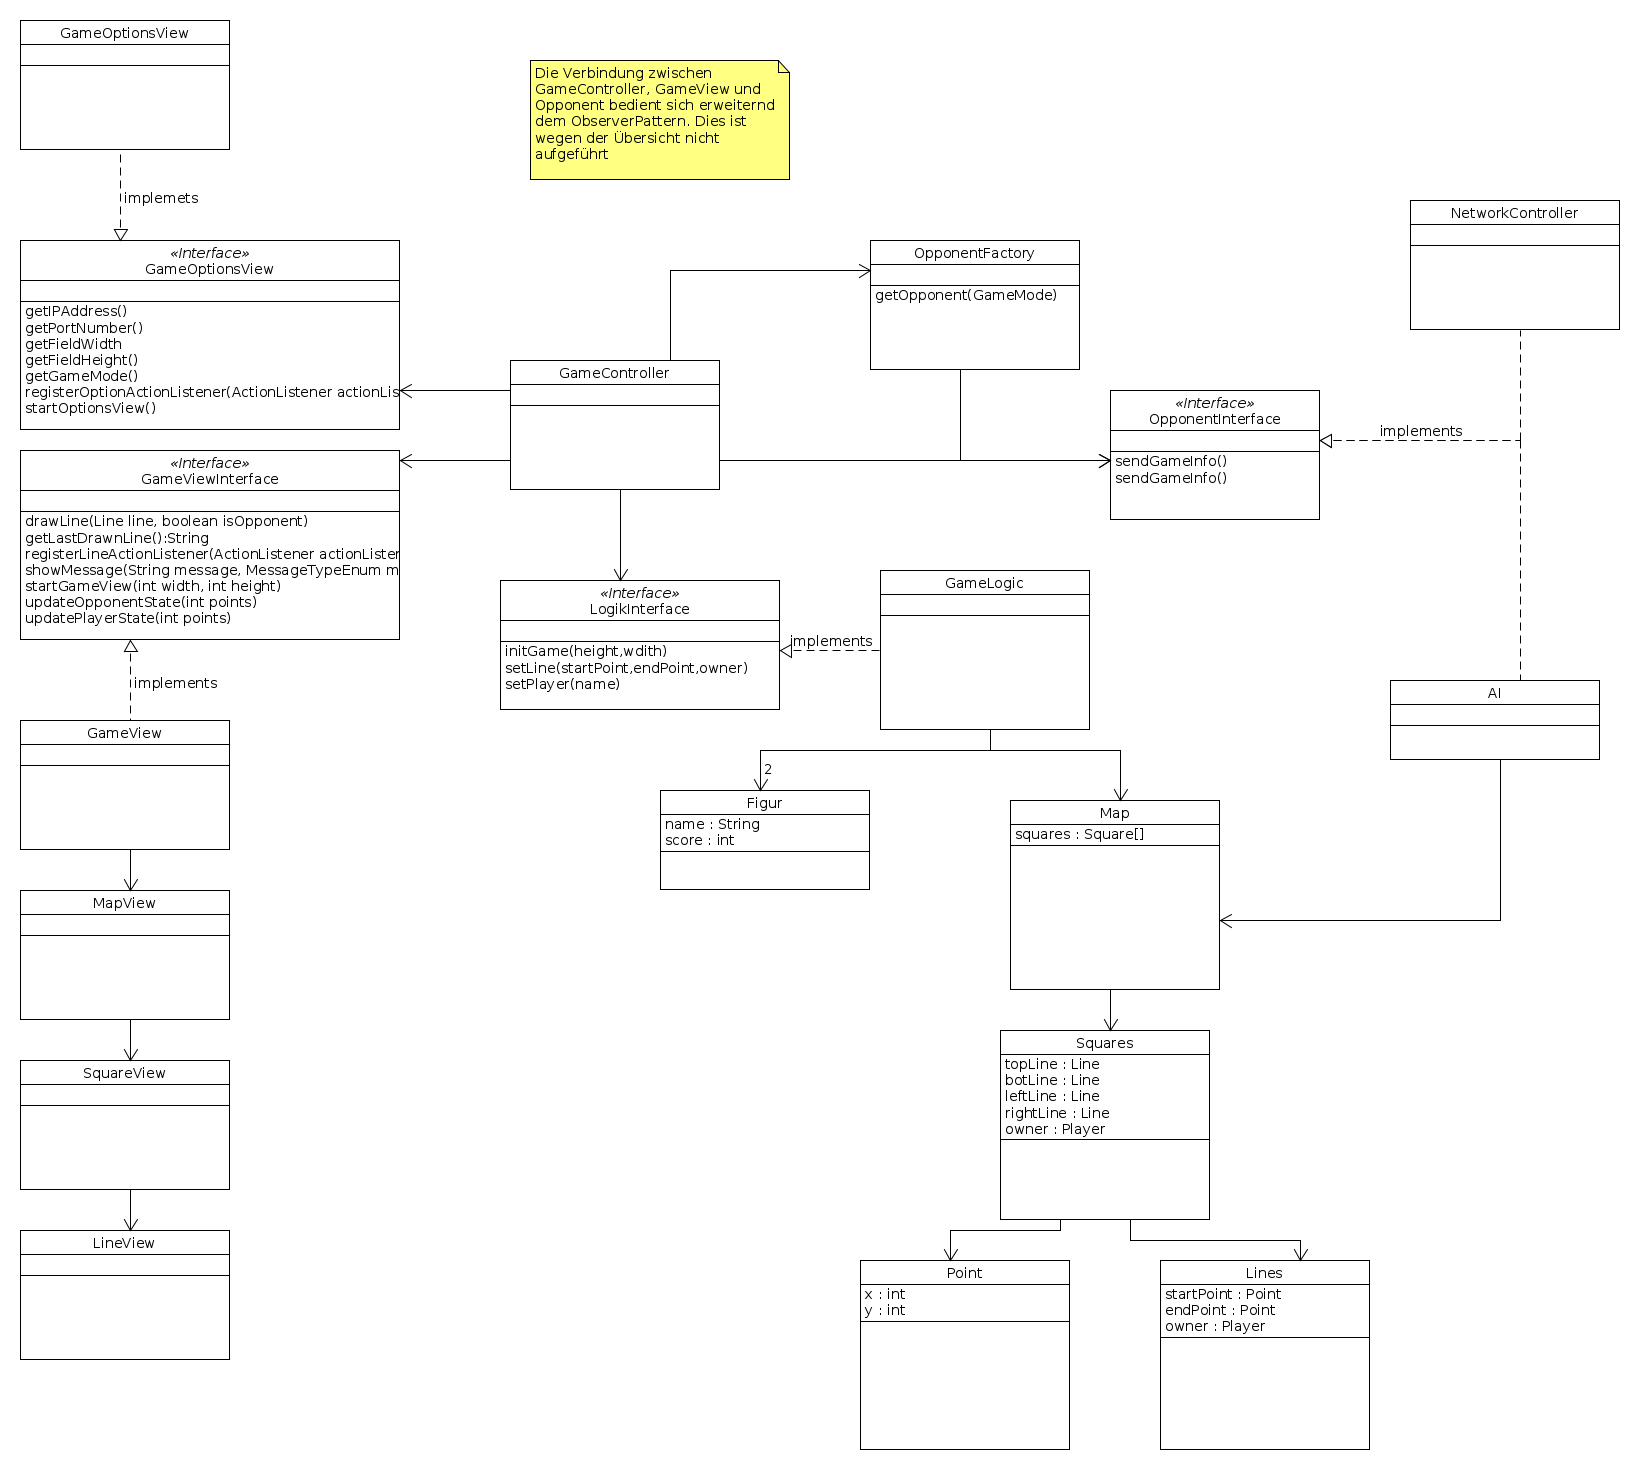
\includegraphics[width=.8\textwidth]{classdiagram.png}
				\caption{class diagram}
			\end{figure}
			\subsubsection{Class Details}
				\begin{description}
					\item[GameController] Der GameController ist für den Datenfluss zwischen GameLogik, View und Netzwerk zuständig.
					\item[GameLogic] Die GameLogic beinhaltet die Regeln von Dots \& Boxes. Sie überprüft die Spielzüge auf ihre Validität und setzt wer als nächster den Zug macht. Sie verwendet zur Datenmodelierung die Klassen \textit{Map, Figur, Squares, Lines} und \textit{Point}
					\item[LogikInterface] definiert die Schnittstelle zwischen GameLogic und GameController
					\item[OpponentFactory] Die OpponentFactory verwendet das Factory Pattern und erstellt eine Klasse basierend auf dem OpponentInterface. Sie erstellt ein Objekt der Klasse NetworkController oder AI
					\item[OpponentInterface] definiert die Schnittstelle zwischen Network/AI und GameController
					\item[AI] Die AI Klasse beinhaltet die ganze Computerspielerlogik.
					\item[GameOptionsView] Die GameOptionsView stellt das GUI zur Eingabe der Optionen dar.
					\item[GameView] Die GameView stellt das Spiel UI dar. Sie verwendet die Klassen \textit{MapView,SquareView} und \textit{LineView} um das Spiel korrekt darzustellen.
					\item[GameViewInterface] definiert die Schnittstelle zwischen GameController und GameView dar.
					\item[GameOptionsViewInterface] definiert die Schnittstelle zwischen GameController und GameOptionsView dar.
				\end{description}
			
	\clearpage
	\section*{Appendix}
		%installation detail, export details or test and IDE setups
		
\end{document}
